\documentclass[../ESOF_notes.tex]{subfiles}

\begin{document}

\section{Part I – Software Reviews \& Inspections}
    \subsection{Verification versus Validation}
        \begin{itemize}
            \item \textbf{Verification – are we building the product right}
                \begin{itemize}
                    \item Ensure (mainly through reviews) that intermediate
                    work products and the final product are “well built”, 
                    i.e., conform to their specifications.
                \end{itemize}
            \item \textbf{Validation – are we building the right product?}
                \begin{itemize}
                    \item Ensure (manly through tests) that the final 
                    product will fulfill its intended use in its intended 
                    environment.
                    \item Can also be applied to intermediate work products, 
                    as predictors of how well the final product will satisfy 
                    user needs.
                \end{itemize}
        \end{itemize}
        Verification shows conformance with specification.
        Validation shows that the program meets the customer’s needs.
        \begin{figure}[h]
            \centering
            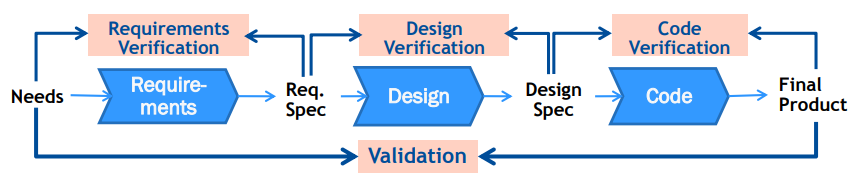
\includegraphics[width=12cm]{Validation_Verification.png}
        \end{figure}

    \subsection{Técnicas V\&V Estáticas e Dinâmicas}
        \begin{itemize}
            \item \textbf{Static Techniques} –– involve analyzing the 
            static system representations to find problems and 
            evaluate quality.
                \begin{itemize}
                    \item Reviews and inspections.
                    \item Automated static analysis (e.g., with lint).
                    \item Formal verification (e.g., with Dafny)
                \end{itemize}
            \item \textbf{Dynamic Techniques} – involve executing the system and
            observing its behavior.
                \begin{itemize}
                    \item Software testing.
                    \item Simulation.
                \end{itemize}
        \end{itemize}
        \paragraph{}
        Static verification techniques involve examination and
        analysis of the program for error detection. Dynamic
        techniques involve executing the program for error
        detection. 
        \paragraph{}
        They are complementary and not opposing techniques.
        Both should be used during the V\&V process.
\pagebreak       
    \subsection{Software reviews and inspections}
        \paragraph{}
        Analysis of static system representations to find problems.
        \begin{itemize}
            \item Manual analysis of requirements specs, 
            design specs, code, etc.
            \item  May be supplemented by tool-based 
            static analysis.
        \end{itemize}
        \paragraph{}
        Advantages (as compared to testing): 
        \begin{itemize}
            \item Can be applied to any artefact, and not only code
            \item Can be applied earlier (thus reducing impact and cost of errors)
            \item Fault localization (debugging) is immediate
            \item Allows evaluating internal quality attributes (e.g., maintainability)
            \item Usually more efficient and effective than testing in finding security
            vulnerabilities and checking exception handling
            \item Very effective in finding multiple defects
            \item Peer reviews promote knowledge sharing
        \end{itemize}

        \subsection{Efficiency of defect removal methods}
            \begin{figure}[h!]
                \centering
                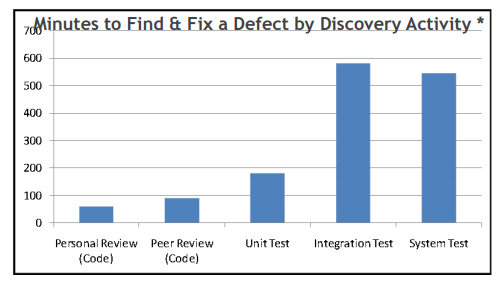
\includegraphics[width=12cm]{minutes_per_defect.png}
            \end{figure}
\pagebreak
        \subsection{Types of Reviews}
            \begin{figure}[h!]
                \centering
                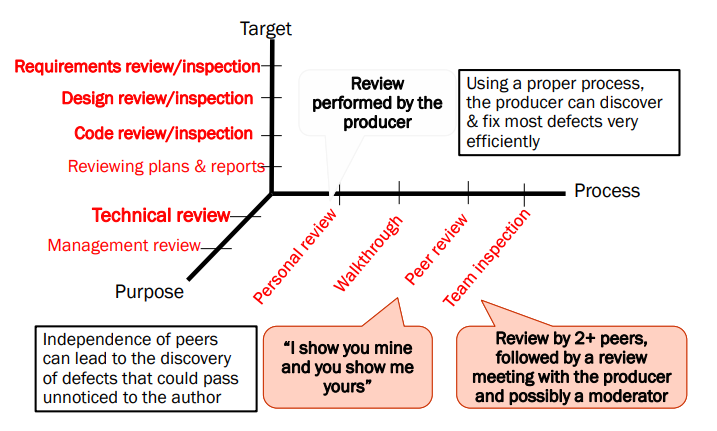
\includegraphics[width=12cm]{type_review.png}
            \end{figure}

        \subsection{Review Best Practices}
            \begin{itemize}
                \item \textbf{Use a checklist derived from historical defect data:} 
                \begin{itemize}
                    \item Makes the review more effective and efficient, by focusing
                    the attention on the most frequent and important problems. 
                    \item CPersonal checklists make sense, because each person
                    tends to repeat his/her own mistakes.
                    
                \end{itemize}
                \item \textbf{Take enough review time :} 200 LOC/hour 
                is a recommended review rate by some authors(LOC-Lines of Code).
                \item \textbf{Take a break between developing and reviewing
                (in personal reviews).}
                \item \textbf{Combine personal reviews with peer reviews or team
                inspections:} Team inspections comprise individual reviews 
                performed by 2+ peers (Individual preparation), followed 
                by a meeting (Inspection meeting) with the producer and 
                possibly a moderator.
                \begin{figure}[h!]
                    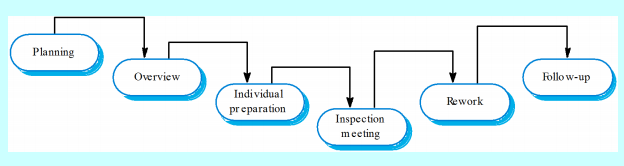
\includegraphics[width=12cm]{inspection_process.png}
                    \centering
                    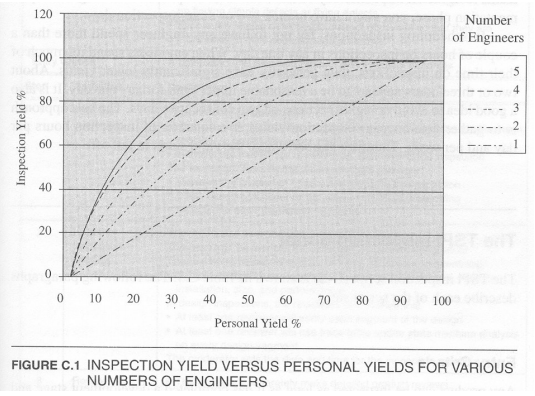
\includegraphics[width=12cm]{defects_found.png}
                \end{figure}
\pagebreak
                \item \textbf{Measure the review process \& use data to improve:} 
                size, time spent, defects found, defects escaped (found later).
            \end{itemize}
\pagebreak
        \subsection{Estimate Missed defects}
        \paragraph{}
        The capture-recapture method is used to estimate the total
        defects (T) and number of defects remaining (R) based on
        the degree of overlapping between defects detected by
        different inspectors (A, B).
        \begin{figure}[h!]
            \centering
            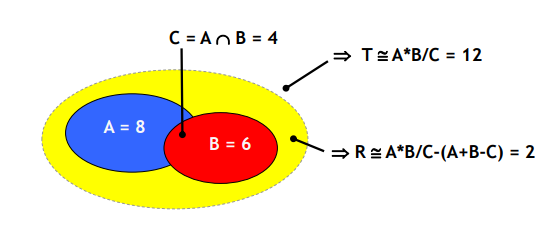
\includegraphics[width=12cm]{capture_recapture.png}
        \end{figure}
        \paragraph{}
        In case of more than 2 inspectors, \textbf{A} refers to the inspector that found
        more unique defects, and \textbf{B} refers to the union of all other inspectors


\section{Part II – Software Testing}
    \subsection{Test Concepts}
        \subsubsection{Testing goals and limitations}
            \paragraph{}
            Goals:
            \begin{itemize}
                \item exercise the software with defined test cases 
                and observe its behaviour to discover defects.
                \item  increase the confidence on the software 
                correctness and to evaluate product quality.
            \end{itemize}
            \paragraph{}
            Limitations:
            \begin{itemize}
                \item Testing can show the presence of bugs, not their absence
            \end{itemize}
        \subsubsection{Test Cases}
            \begin{itemize}
                \item \textbf{Test Case:} A set of test inputs, 
                execution conditions, and expected results developed
                to exercise a particular program path.
                \item \textbf{Test Script:} concrete definition of test 
                steps / procedure( can be parameterized for reuse with 
                multiple test data).
            \end{itemize}
        \subsubsection{Test Activities}
            \begin{itemize}
                \item \textbf{Test Planning:} define the objectives of 
                testing and the approach for meeting test objectives 
                within constraints imposed by the context.
                \item \textbf{Test monitoring and control:} compare actual 
                progress against the plan, and take actions necessary 
                to meet the objectives of the test plan.
                \item \textbf{Test analysis:} identify testable features 
                and test conditions.
                \item \textbf{Test design:} derive test cases.
                \item \textbf{Test implementation:} create automated scripts.
                \item \textbf{Test execution:} run test suites.
                \item \textbf{Test completion:} collect data from completed 
                test activities.
            \end{itemize}
        \subsubsection{Test Types}
        \begin{figure}[h!]
            \centering
            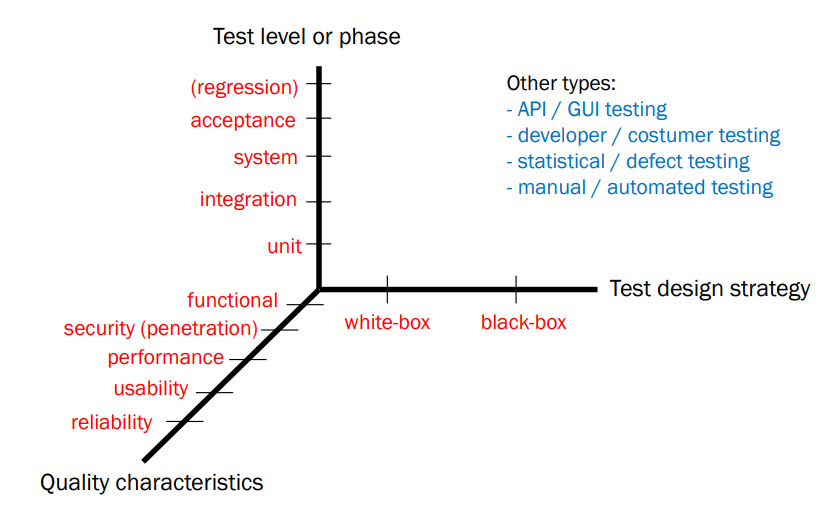
\includegraphics[width=12cm]{test_types.png}
        \end{figure}
    \subsection{Test Levels}
        \subsubsection{Unit Testing/Component Testing/Module Testing}
            \begin{itemize}
                \item Testing of individual hardware or software units or 
                groups of related units.
                \item Detect functional (e.g., wrong calculations) 
                and non-functional (e.g., memory leaks) defects in 
                the unit.
                \item Usually API testing.
                \item Responsibility of the developer.
                \item Usually based on experience, specs and code.
            \end{itemize}
        \subsubsection{Integration Testing}
            \begin{itemize}
                \item Software and/or hardware components are
                combined and tested to evaluate the interaction
                 between them.
                \item Two levels of integration testing:
                    \begin{itemize}
                        \item \textbf{Component integration testing:} 
                        interactions between components.
                        \item \textbf{System integration testing:}
                        interactions between systems.
                    \end{itemize} 
                \item Responsibility of an independent test team.
                \item Usually based on a system spec (technical/design spec).
                \item Detect defects that occur on the units’ interfaces.
                \item For easier fault localisation, integrate 
                incrementally/continuously.
            \end{itemize}
        \subsubsection{System Testing}
            \begin{itemize}
                \item Conducted on a complete, integrated system 
                to evaluate the system's compliance with specified 
                requirements.                
                \item Both functional behavior and quality requirements
                (performance, usability, reliability, security, etc.) 
                are evaluated.   
                \item Usually GUI testing.
                \item Responsibility of an independent test team.
                \item Usually based on requirements document.
            \end{itemize}
        \subsubsection{Acceptance Testing}
        \begin{itemize}
            \item Determine whether or not a system atisfies its 
            acceptance criteria.
            \item Enable a customer,user, or other authorized entity 
            to determine whether or not to accept the system.
            \item Usually the responsibility of the customer.
            \item Based on a requirements document or contract.
            \item Check if customer requirements and expectations 
            are met.
        \end{itemize}
        \subsubsection{Regression Testing}
            \begin{itemize}
                \item Tests to verify that modifications have not
                caused unintended effects and that the system or 
                component still complies with its specified requirements.
                \item Changes to software, to enhance it or fix bugs,
                are a very common source of defects.
                \item Not really a new test level, but just the repetition
                of testing at any level.
            \end{itemize}
    \subsection{Test case design techniques}
            \subsubsection{Design goals:}
            \begin{itemize}
                \item Create a set of test cases (test suite) that are 
                effective in validation and defect testing.
                \item A good test suite should have a small/manageable 
                size and have a high probability of finding most of the 
                defects.
            \end{itemize}
            \subsubsection{Design Strategies:}
            \paragraph{}
            \textbf{Black-Box Testing:} Derivation of test 
            cases based on some external specification.
            \begin{itemize}
                \item \textbf{Equivalence class partitioning:} 
                partition the input domain into classes of equivalent 
                behavior, separating classes of valid and invalid 
                inputs, and select at least one test case from each
                class.
                \item \textbf{Boundary value analysis:} select test 
                values at the boundaries of each partition 
                (e.g., immediately below and above), besides typical 
                values.
                \item \textbf{Decision table testing:} test all possible 
                combinations of a set of conditions and actions 
                (each combination corresponding to a business rule). 
                \item \textbf{State transition testing:} derive test 
                cases from a state-machine model of the system.
                \item \textbf{Use case testing:} derive test cases 
                from a use case model of the system (with use cases 
                possibly detailed with scenarios, pre/post-conditions, 
                etc).
            \end{itemize}
            \paragraph{}
            \textbf{White-box Testing:} Derivation of test 
            cases according to program structure.
            \begin{itemize}
                \item \textbf{Using coverage analysis tools:} (e.g., Eclemma)
                to analyse code coverage achieved by black-box tests
                and design additional tests as needed.
                \item  \textbf{Testing statement coverage:} Assure that 
                all statements are exercised.
                \item \textbf{Decision/Branch coverage:} Assure that all decisions
                (if, while, for, etc.) take both values true and false. 
            \end{itemize} 
    \subsection{Test automation tools}
    \begin{itemize}
        \item \textbf{Unit testing frameworks:} JUnit, NUnit.
        \item \textbf{Mock object frameworks:}
        \begin{itemize}
            \item Facilitate simulating external components in unit testing.
            \item EasyMock, jMock.
        \end{itemize}
        \item \textbf{Test coverage analysis tools:}
        \begin{itemize}
            \item Measure degree of code coverage 
            achieved by the execution of a test suite.
            \item Useful for white-box testing.
            \item Eclemma, Clover.
        \end{itemize}
        \item \textbf{Mutation testing tools:}
        \begin{itemize}
            \item Evaluate the quality of a test suite by 
            determining its ability to ‘kill’ mutants
            (with common fault types) of the program under test.
            \item pitest, muJava.
        \end{itemize}
        \item \textbf{Acceptance testing frameworks:}
        \begin{itemize}
            \item Allows creating test cases by people 
            without technical knowledge.
            \item Cucumber, JBehave, Fitnesse.
        \end{itemize}
        \item \textbf{Capture/replay tools (aka functional testing tools):}
        \begin{itemize}
            \item Capture user interactions in scripts 
            that can be edited and replayed.
            \item Useful for GUI testing, particularly 
            regression testing.
            \item Selenium, IBM Rational Functional Tester.
        \end{itemize}
        \item \textbf{Performance/load testing tools:}
        \begin{itemize}
            \item Execute test suites simulating many users
            and measure system performance.
            \item IBM Rational Performance Tester, Compuware QA Load.
        \end{itemize}
        \item \textbf{Penetration testing tools:} Metasploit, ZAP.
        \item \textbf{Test case generation tools:}
        \begin{itemize}
            \item Automatically generate test cases from 
            models or code.
            \item IParTeG (UML), EvoSuite (Java), Spec Explorer (Spec\#),
             Conformiq (UML).
        \end{itemize}
    \end{itemize}
    \subsection{Test management}
    \paragraph{}
    Tools:
    \begin{itemize}
        \item Manage test information and status.
        \item Integrate with other management tools: 
        requirements management, project management, 
        bug tracking, configuration management.
        \item Integrate with test automation tools.
        \item TestLink.
    \end{itemize}
    \paragraph{}
    Test Management charts are used to track progress 
    of testing and bug fixing activities.

    \subsection{Testing best practices}
    \begin{itemize}
        \item \textbf{Test as early as possible} The cost of finding
        and fixing bugs increases exponentially with time.
        \item \textbf{Automate the tests}.
        \item \textbf{Test first (write tests before the code):}
        Helps clarifying requirements and specifications since
        test cases are partial specifications of system behavior.
        \item \textbf{Black-box first:} Start by designing test 
        cases based on the specification and then add any tests 
        needed to ensure code coverage.
    \end{itemize}
\pagebreak
    \subsection{Useful Kahoots}
    \begin{figure}[h!]
        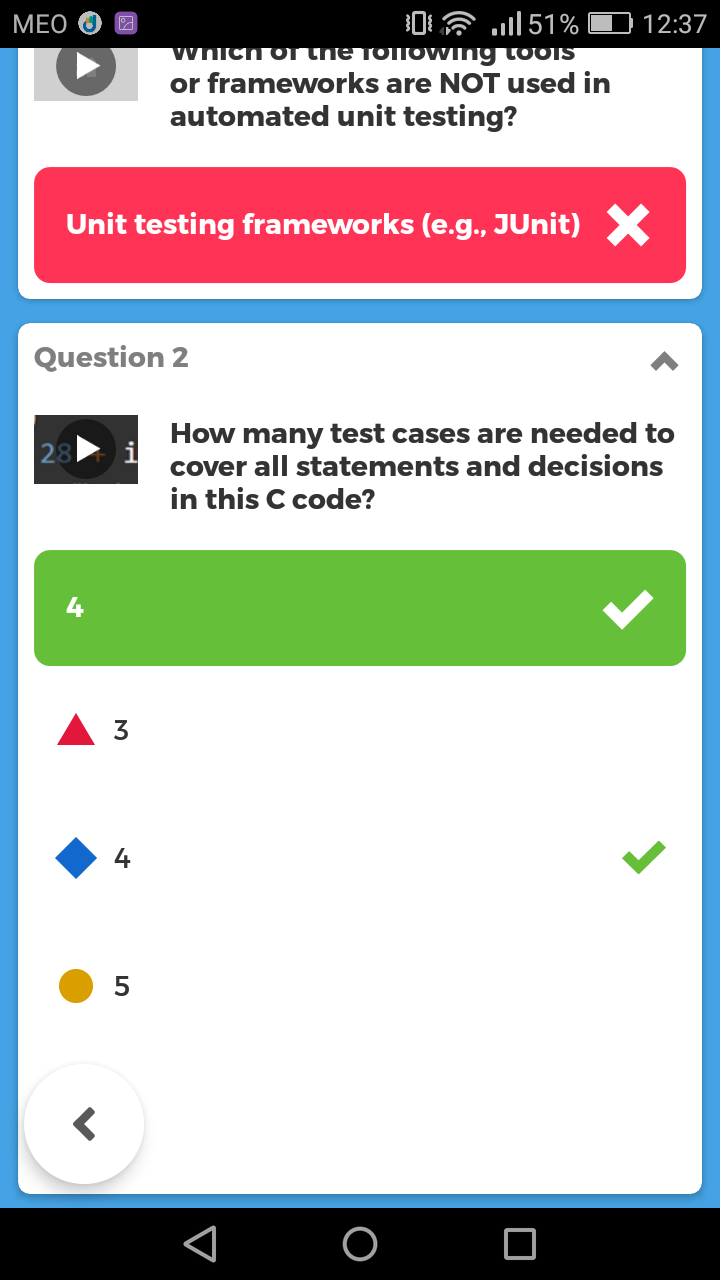
\includegraphics[width=4cm]{ST-11_1.png}
        \centering
        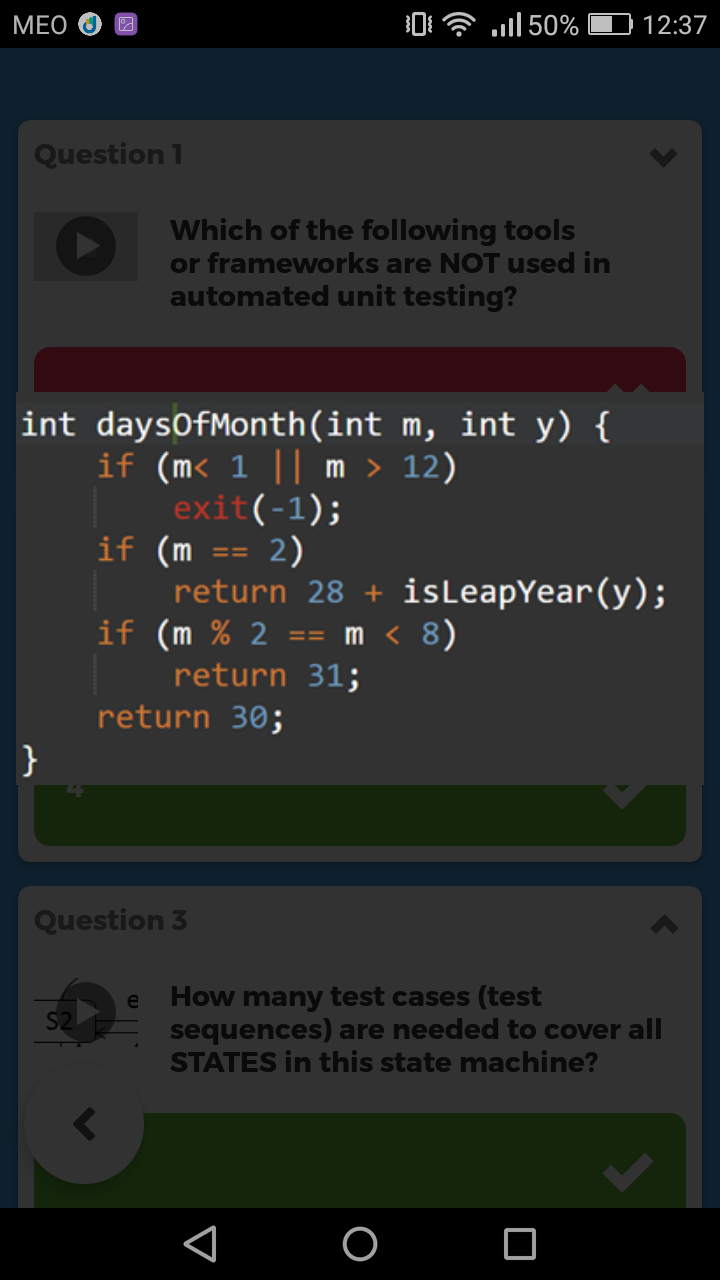
\includegraphics[width=4cm]{ST-11_2.png}
        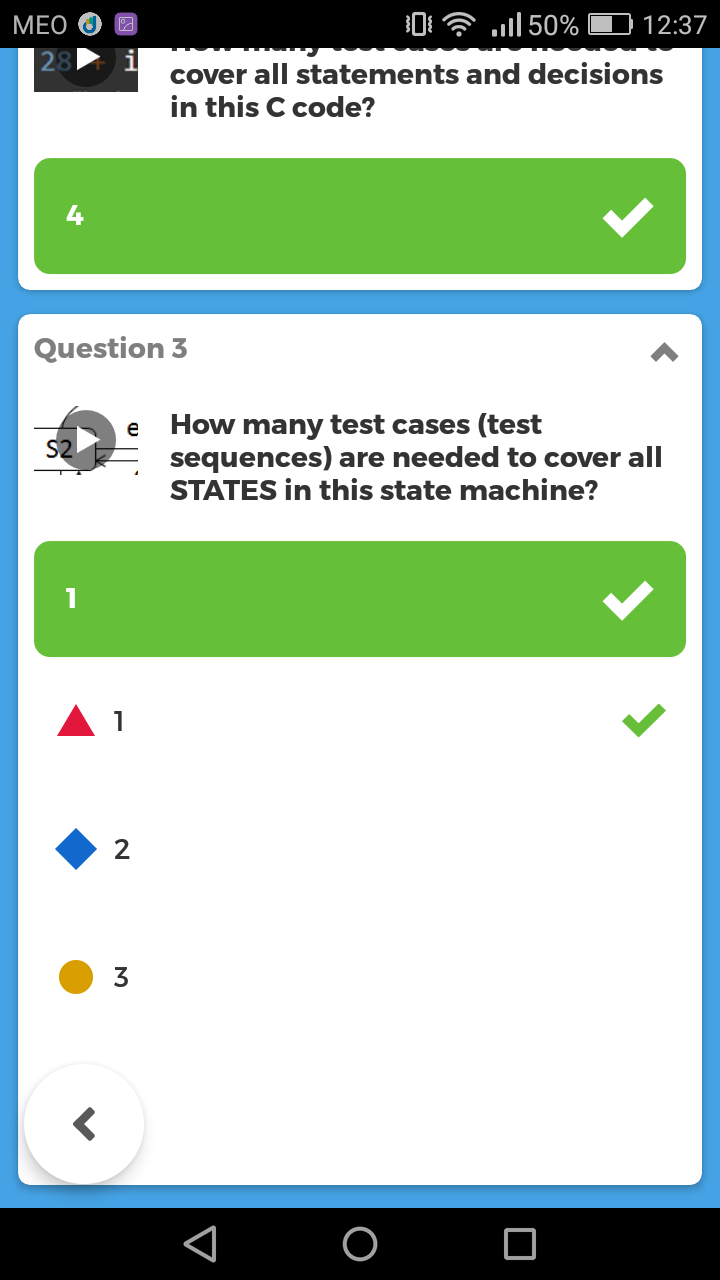
\includegraphics[width=4cm]{ST-12_2.png}
        \centering
        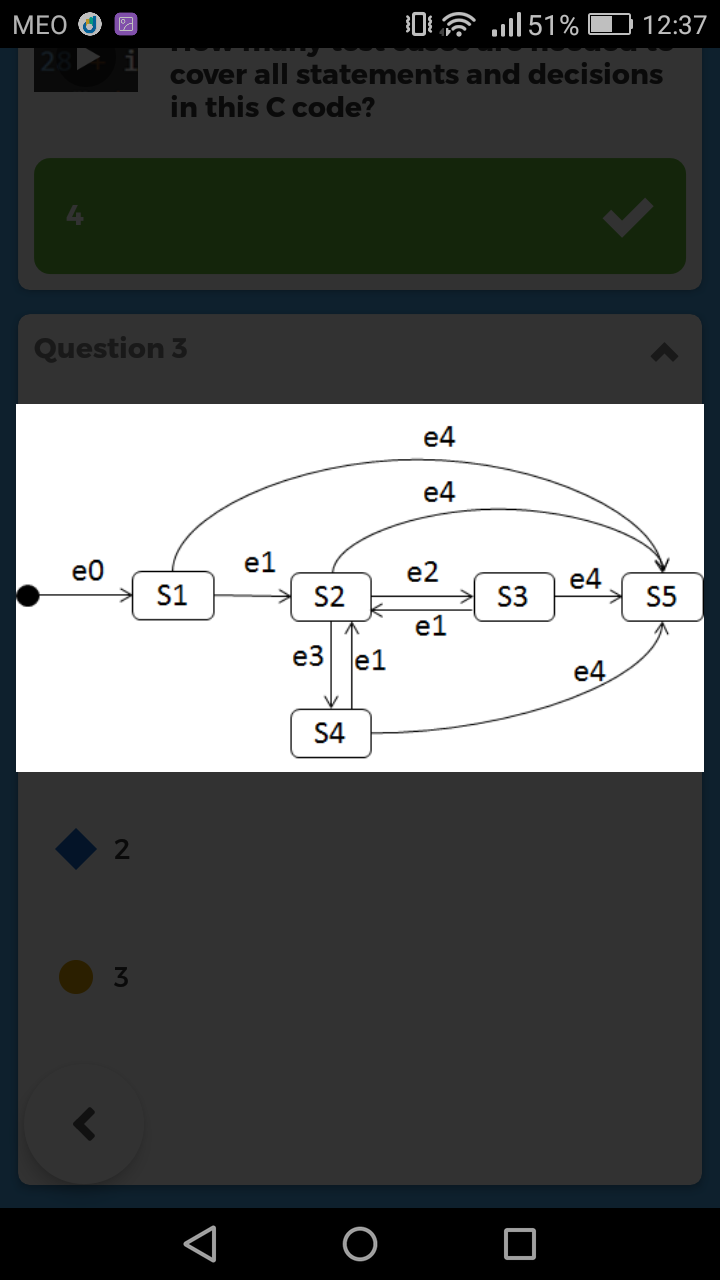
\includegraphics[width=4cm]{ST-12_1.png}
    \end{figure}
\end{document}